\documentclass{beamer}
\usepackage{boondox-calo} % lowercase calligraphic letters
\usepackage[backend=biber]{biblatex}
\usepackage{optidef}

\beamertemplatenavigationsymbolsempty
\usetheme{Warsaw}
\addbibresource{reference.bib}
\setbeamertemplate{bibliography item}{\insertbiblabel}

\renewcommand{\bibfont}{\tiny}

\renewcommand
{\vec}
[1]
{\boldsymbol{\mathbf{#1}}}

\newcommand
{\const}
{\mathfrak}

\newcommand
{\embbRa} % eMBB resource allocation
{\alpha}

\newcommand
{\urllcRa}
{\beta}

\newcommand
{\embb}
{\vec{\embbRa}}

\newcommand
{\urllc}
{\vec{\urllcRa}}

\newcommand
{\embbTwo}
[2]
{\embbRa_{#1, #2}}

\newcommand
{\lossFunc}
[1]
{f( #1 )}

\newcommand
{\proportion}
{x}

\newcommand
{\embbThree}
[3]
{\embbRa_{#1, #2, #3}}

\newcommand
{\embbFour}
[4]
{\embbRa_{#1, #2, #3, #4}}

\newcommand
{\embbMini}
[3]
{\embbRa_{#1, #2, #3}}

\newcommand
{\urllcUser}
{v_{0}}

\newcommand
{\urllcFour}
[4]
{\urllcRa_{#1, #2, #3, #4}}

\newcommand
{\urllcFive}
[5]
{\urllcRa_{#1, #2, #3, #4, #5}}

\newcommand
{\urllcThreeBug}
[3]
{\urllcRa_{#1, #2, #3}}

\newcommand
{\urllcFourBug}
[4]
{\urllcRa_{#1, #2, #3, #4}}

\newcommand
{\urllcTime}
{m}

\newcommand
{\urllcTimeN}
{\const{\urllcTime}}

\newcommand
{\urllcDemand}
{D}

\newcommand
{\ex}
{\mathbb{E}}

\newcommand
{\demandOne}
[1]
{\urllcDemand_{#1}}

\newcommand
{\demandTwo}
[2]
{\urllcDemand_{#1, #2}}

\newcommand
{\demandThree}
[3]
{\urllcDemand_{#1, #2, #3}}

\newcommand
{\peakRate}
[3]
{\const{\rate}_{#1, #2, #3}}

\newcommand
{\peakRateTwo}
[2]
{\const{\rate}_{#1, #2}}

\newcommand
{\embbUserN}
{\const{\embbUser}}

\newcommand
{\rateThree}
[3]
{\rate_{#1, #2, #3}}

\newcommand
{\embbUser}
{u}

\newcommand
{\embbTime}
{n}

\newcommand
{\embbTimeN}
{\const{\embbTime}}

\newcommand
{\subchannel}
{l}

\newcommand
{\subchannelN}
{\const{\subchannel}}

\newcommand
{\rate}
{r}

\newcommand
{\avgRate}
[1]
{\bar{\rate_{#1}}}

\newcommand
{\rateTwo}
[2]
{\rate_{#1, #2}}

\newcommand
{\factorRa}
{\gamma}

\newcommand
{\factorThree}
[3]
{\factorRa_{#1, #2, #3}}

\title{Joint Scheduling of URLLC and eMBB Traffic in 5G Wireless Networks}
\author{Arjun Anand, Gustavo de Veciana, and Sanjay Shakkottai}
\institute{Department of Electrical and Computer Engineering, The University of Texas at Austin, Austin, USA}
\date{April, 2020}

\begin{document}

\begin{frame}
  \titlepage
  Published in IEEE/ACM Transactions on Networking (also in IEEE INFOCOM 2018)
\end{frame}

\begin{frame}
  \frametitle{System Model}
  \begin{itemize}
    \item Saturated system \cite{S05}: Each eMBB user has infinite amount of data to be served.
  \end{itemize}
  \begin{figure}
    \includegraphics[width=0.7\textwidth]{system_model}
    \caption{System model}
  \end{figure}
\end{frame}

\begin{frame}
  \frametitle{System Framework}
  \begin{figure}
    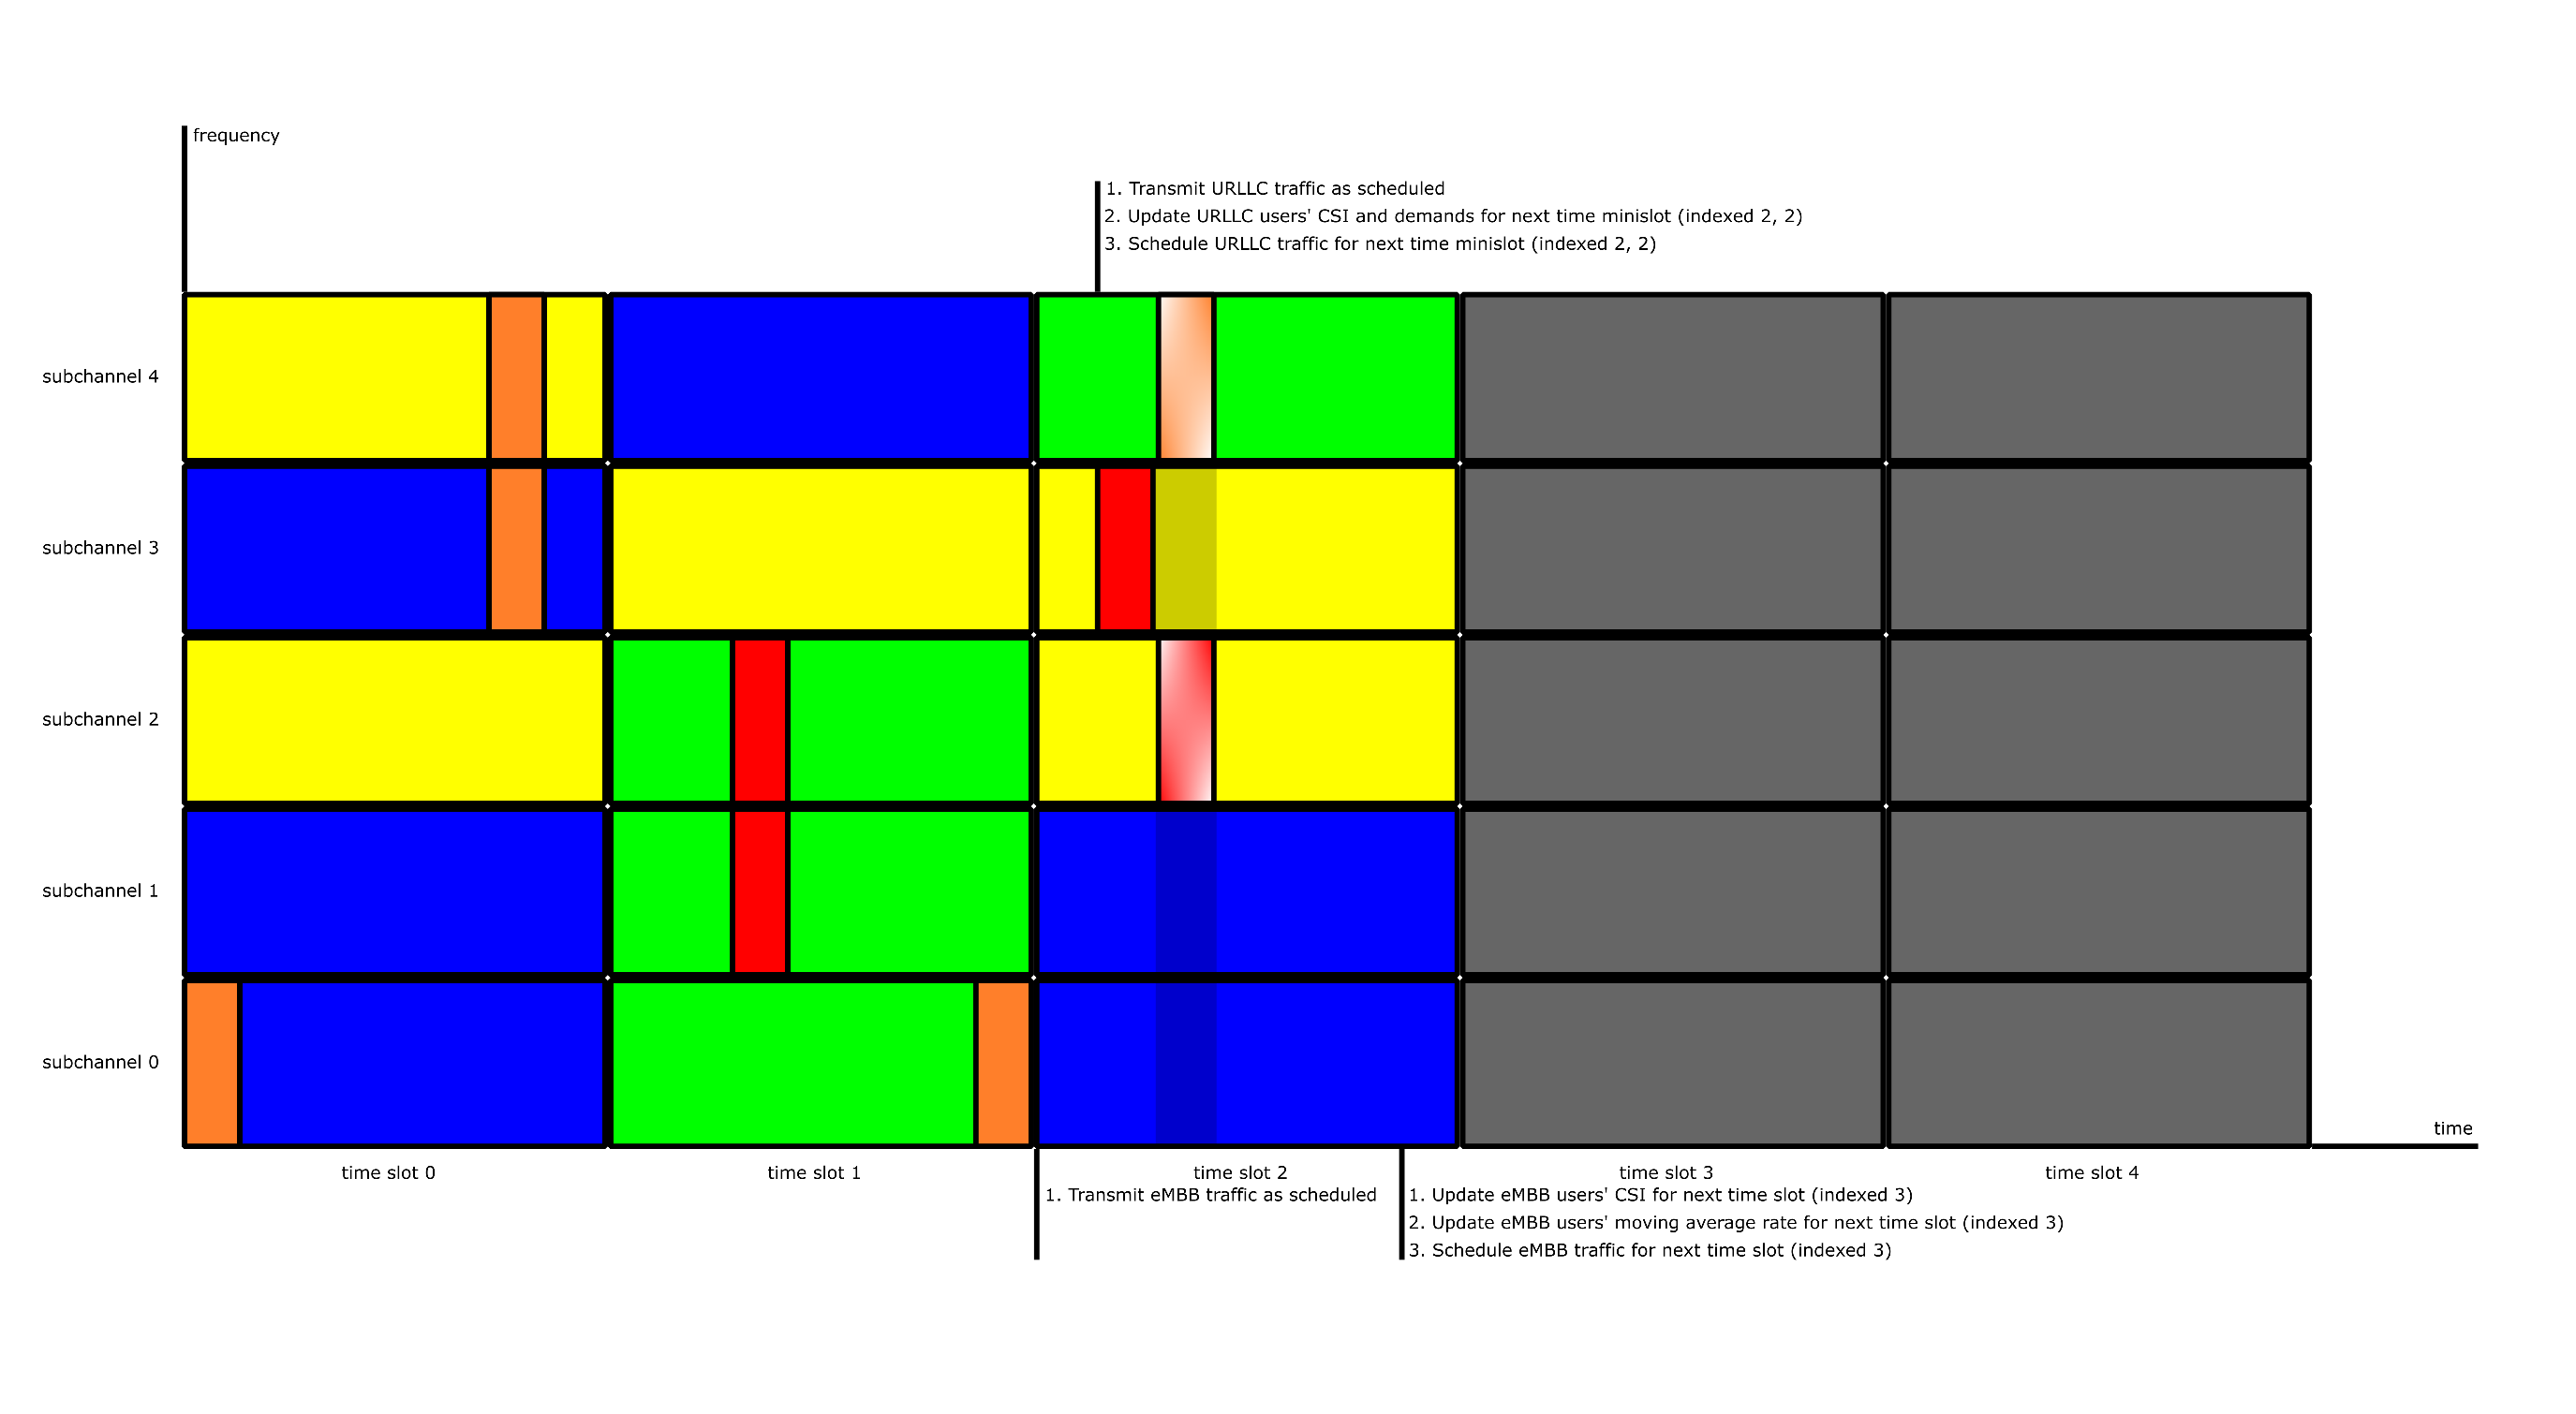
\includegraphics[width=\textwidth]{system_framework}
    \caption{System framework \cite{YZR21}}
  \end{figure}
\end{frame}

\begin{frame}
  \frametitle{Problem Statement}
  \begin{itemize}
    \item URLLC puncturing/superposition commonly used scheduling procedure: allocate \emph{subchannels} for eMBB users in the given time slot first, then schedule \emph{resources} for URLLC users in the respective time minislots accordingly.
    \item Multiplexing -- conducting eMBB resource allocation using only eMBB channel state information (CSI) -- has been broadly discussed in the literature.
    \item However, joint scheduling of eMBB and URLLC traffics has not been well studied.
    \item That is, in addition to eMBB CSI, could we also leverage URLLC information (e.g. \emph{observed} behavior of URLLC demands, any others?) to schedule eMBB?
  \end{itemize}
\end{frame}

\begin{frame}
  \frametitle{Examples}
  \begin{itemize}
    \item Discussion with Yung-Ching senpai: Reduce eMBB retransmissions of data damaged by URLLC puncturing/superposition.
      \begin{itemize}
        \item Approach 1: Reserve resources for URLLC traffic.
        \item Approach 2: Pre-allocate resources for some URLLC users (less overhead compared to the first method, which increases URLLC reliability).
      \end{itemize}
    \item However, their paper does not address the aforementioned problems, but aims to tackle two questions:
      \begin{itemize}
        \item For linear loss model, would the traditional multiplexing procedure be optimal in the long-term?
        \item For convex loss model, could we somehow incorporate URLLC demands into eMBB resource allocation formulation?
      \end{itemize}
  \end{itemize}
\end{frame}

\begin{frame}
  \frametitle{Solution}
  \begin{itemize}
    \item The main idea is to perform mathematical analysis on eMBB time slot.
    \item This is done by their model `proportion of an eMBB time slot's resource'.
    \item Linear, convex, and threshold loss models are discussed.
  \end{itemize}
\end{frame}

\begin{frame}
  \frametitle{Linear Loss Model}
  \begin{itemize}
    \item A URLLC \emph{puncturing} problem is formulated as follows:
      \begin{maxi}
        { \embb, \urllc }{ \sum_{ \embbUser }{ ln\left( \avgRate{\embbUser} \right) } }
        {\label{pb:linear}}{}
        \addConstraint
          { \sum_{ \embbUser }{ \embbThree{\embbUser}{\embbTime}{\subchannel} } }
          { \leq \frac{ 1 }{ \subchannelN },\quad }
          { \forall\embbTime, \forall\subchannel }
        \addConstraint
          { \embbThree{\embbUser}{\embbTime}{\subchannel} }
          { \in \left\{ 0, \frac{ 1 }{ \subchannelN } \right\},\quad }
          { \forall\embbUser, \forall\embbTime, \forall\subchannel }
        \addConstraint
          { \sum_{ \embbUser }{ \sum_{ \subchannel }{ \urllcFive{\urllcUser}{\embbUser}{\embbTime}{\urllcTime}{\subchannel} } } }
          { = \demandThree{\urllcUser}{\embbTime}{\urllcTime},\quad }
          { \forall\embbTime, \forall\urllcTime }
        \addConstraint
          { \urllcFive{\urllcUser}{\embbUser}{\embbTime}{\urllcTime}{\subchannel} }
          { \leq \embbFour{\embbUser}{\embbTime}{\urllcTime}{\subchannel},\quad }
          { \forall\embbUser, \forall\embbTime, \forall\urllcTime, \forall\subchannel }
        \addConstraint
          { \urllcFive{\urllcUser}{\embbUser}{\embbTime}{\urllcTime}{\subchannel} }
          { \in \left\{ 0, \frac{ 1 }{ \urllcTimeN \subchannelN } \right\},\quad }
          { \forall\embbUser, \forall\embbTime, \forall\urllcTime, \forall\subchannel }
    \end{maxi}
    \item where
      \begin{equation}
        \embbFour{\embbUser}{\embbTime}{\urllcTime}{\subchannel} = \frac{ \embbThree{\embbUser}{\embbTime}{\subchannel} }{ \urllcTimeN },\quad \forall\embbUser,\forall\embbTime,\forall\urllcTime,\forall\subchannel
      \end{equation}
  \end{itemize}
\end{frame}

\begin{frame}
  \frametitle{Linear Loss Model (Continued)}
  \begin{itemize}
    \item The average rate is calculated as follows.
      \begin{align}
        \avgRate{\embbUser} & = \frac{ \rateTwo{\embbUser}{0} + \rateTwo{\embbUser}{1} + \ldots + \rateTwo{\embbUser}{\embbTimeN - 1} }{ \embbTimeN }\\
                            & = \frac{ 1 }{ \embbTimeN } \sum_{ \embbTime }{ \rateTwo{\embbUser}{\embbTime} }\\
                            & = \frac{ 1 }{ \embbTimeN } \sum_{ \embbTime }{ \sum_{ \subchannel }{ \rateThree{\embbUser}{\embbTime}{\subchannel} } }\\
                            & = \frac{ 1 }{ \embbTimeN } \sum_{ \embbTime }{ \sum_{ \subchannel }{ \left( \embbThree{\embbUser}{\embbTime}{\subchannel} - \urllcFour{\urllcUser}{\embbUser}{\embbTime}{\subchannel} \right) \peakRate{\embbUser}{\embbTime}{\subchannel} } },\quad \forall\embbUser
      \end{align}
    \item In this paper, subchannel allocation is neglected.
      \begin{align}
        \avgRate{\embbUser} & = \frac{ 1 }{ \embbTimeN } \sum_{ \embbTime }{ \rateTwo{\embbUser}{\embbTime} }\\
                            & = \frac{ 1 }{ \embbTimeN } \sum_{ \embbTime }{ \left( \embbTwo{\embbUser}{\embbTime} - \urllcThreeBug{\urllcUser}{\embbUser}{\embbTime} \right) \peakRateTwo{\embbUser}{\embbTime} },\quad \forall\embbUser
      \end{align}
  \end{itemize}
\end{frame}

\begin{frame}
  \frametitle{Linear Loss Model (Continued)}
  \begin{itemize}
    \item The first idea that comes to my mind is to give each eMBB user an equal share of URLLC demands.
      \begin{equation}
        \urllcFourBug{\urllcUser}{\embbUser}{\embbTime}{\urllcTime} = \frac{ \demandThree{\urllcUser}{\embbTime}{\urllcTime} }{ \embbUserN },\quad \forall\embbUser, \forall\embbTime, \forall\urllcTime
      \end{equation}
    \item However, this cannot guarantee
      \begin{equation}
        \urllcFourBug{\urllcUser}{\embbUser}{\embbTime}{\urllcTime} \leq \embbMini{\embbUser}{\embbTime}{\urllcTime},\quad \forall\embbUser, \forall\embbTime, \forall\urllcTime.
      \end{equation}
    \item It is then intuitive to give each eMBB user a proportionally equal share of URLLC demands.
      \begin{align}
        \urllcFourBug{\urllcUser}{\embbUser}{\embbTime}{\urllcTime} & = \frac{ \embbMini{\embbUser}{\embbTime}{\urllcTime} }{ \frac{ 1 }{ \urllcTimeN } } \demandThree{\urllcUser}{\embbTime}{\urllcTime}\\
                                                                    & = \embbTwo{\embbUser}{\embbTime} \demandThree{\urllcUser}{\embbTime}{\urllcTime}
      \end{align}
  \end{itemize}
\end{frame}

\begin{frame}
  \frametitle{Linear Loss Model (Continued)}
  \begin{itemize}
    \item Such an allocation guarantees URLLC constraints:
      \begin{align}
          \sum_{ \embbUser }{ \urllcFourBug{\urllcUser}{\embbUser}{\embbTime}{\urllcTime} } & = \demandThree{\urllcUser}{\embbTime}{\urllcTime},\quad \forall\embbTime, \forall\urllcTime,\\
          \urllcFourBug{\urllcUser}{\embbUser}{\embbTime}{\urllcTime} & \leq \embbMini{\embbUser}{\embbTime}{\urllcTime},\quad \forall\embbUser, \forall\embbTime, \forall\urllcTime.
      \end{align}
  \end{itemize}
\end{frame}

\begin{frame}
  \frametitle{Linear Loss Model (Continued)}
  \begin{itemize}
    \item URLLC allocation in eMBB time slot can then be derived:
      \begin{align}
        \urllcThreeBug{\urllcUser}{\embbUser}{\embbTime} & = \sum_{ \urllcTime }{ \urllcFourBug{\urllcUser}{\embbUser}{\embbTime}{\urllcTime} }\\
                                                         & = \embbTwo{\embbUser}{\embbTime} \sum_{ \urllcTime }{ \demandThree{\urllcUser}{\embbTime}{\urllcTime} }\\
                                                         & = \embbTwo{\embbUser}{\embbTime} \demandTwo{\urllcUser}{\embbTime}
      \end{align}
  \end{itemize}
\end{frame}

\begin{frame}
  \frametitle{Linear Loss Model (Continued)}
  \begin{block}{Theorem 1}
    For a wireless system under the linear superposition/puncturing loss model we have that $C = C^{LR}$
  \end{block}
  \begin{itemize}
    \item By this theorem, the proportionally equal share policy is optimal.
      \begin{align}
        \avgRate{\embbUser} & = \frac{ 1 }{ \embbTimeN } \sum_{ \embbTime }{ \left( \embbTwo{\embbUser}{\embbTime} - \embbTwo{\embbUser}{\embbTime} \demandTwo{\urllcUser}{\embbTime} \right) \peakRateTwo{\embbUser}{\embbTime} }\\
                            & = \frac{ 1 }{ \embbTimeN } \sum_{ \embbTime }{ \left( 1 - \demandTwo{\urllcUser}{\embbTime} \right) \embbTwo{\embbUser}{\embbTime} \peakRateTwo{\embbUser}{\embbTime} },\quad \forall\embbUser
      \end{align}
    \item Do note that URLLC allocation disappears from the objective function of Problem \ref{pb:linear}, and URLLC demands are constants.
  \end{itemize}
\end{frame}

\begin{frame}
  \frametitle{Linear Loss Model (Continued)}
  \begin{itemize}
    \item This problem then can be solved with gradient algorithm \cite{S05}.
      \begin{maxi}
        { \embb }{ \sum_{ \embbUser }{ ln\left( \avgRate{\embbUser} \right) } }
        {}{}
        \addConstraint
          { \sum_{ \embbUser }{ \embbThree{\embbUser}{\embbTime}{\subchannel} } }
          { \leq \frac{ 1 }{ \subchannelN },\quad }
          { \forall\embbTime, \forall\subchannel }
        \addConstraint
          { \embbThree{\embbUser}{\embbTime}{\subchannel} }
          { \in \{ 0, \frac{ 1 }{ \subchannelN } \},\quad }
          { \forall\embbUser, \forall\embbTime, \forall\subchannel }
      \end{maxi}
    \item However, this paper does not execute two problem transformations required to apply the above algorithm.
  \end{itemize}
\end{frame}

\begin{frame}
  \frametitle{Convex Loss Model}
  \begin{itemize}
    \item Recall that
      \begin{align}
        \avgRate{\embbUser} & = \frac{ 1 }{ \embbTimeN } \sum_{ \embbTime }{ \rateTwo{ \embbUser }{ \embbTime } }\\
                            & = \frac{ 1 }{ \embbTimeN } \sum_{ \embbTime }{ \left( \embbTwo{\embbUser}{\embbTime} - \embbTwo{\embbUser}{\embbTime} \lossFunc{\proportion} \right) \peakRateTwo{\embbUser}{\embbTime} }
      \end{align}
    \item where $\lossFunc{\cdot}$ is a convex function, and
      \begin{equation}
        \proportion = \frac{ \urllcThreeBug{\urllcUser}{\embbUser}{\embbTime} }{ \embbTwo{\embbUser}{\embbTime} }
      \end{equation}
    \item Thus
      \begin{equation}
        \avgRate{\embbUser} = \frac{ 1 }{ \embbTimeN } \sum_{ \embbTime }{ \left( \embbTwo{\embbUser}{\embbTime} - \embbTwo{\embbUser}{\embbTime} \lossFunc{ \frac{ \sum_{ \urllcTime }{ \urllcFourBug{\urllcUser}{\embbUser}{\embbTime}{\urllcTime} } }{ \embbTwo{\embbUser}{\embbTime} } } \right) \peakRateTwo{\embbUser}{\embbTime} },\quad \forall\embbUser
      \end{equation}
  \end{itemize}
\end{frame}

\begin{frame}
  \frametitle{Convex Loss Model (Continued)}
  \begin{itemize}
    \item They first fluidize the bandwidth:
      \begin{maxi}
        { \embb, \urllc }{ \sum_{ \embbUser }{ ln\left( \avgRate{\embbUser} \right) } }
        {}{}
        \addConstraint
          { \sum_{ \embbUser }{ \embbTwo{\embbUser}{\embbTime} } }
          { \leq 1 }
          { \forall\embbTime }
        \addConstraint
          { \embbTwo{\embbUser}{\embbTime} }
          { \geq 0 }
          { \forall\embbUser, \forall\embbTime }
        \addConstraint
          { \sum_{ \embbUser }{ \urllcFourBug{\urllcUser}{\embbUser}{\embbTime}{\urllcTime} } }
          { = \demandThree{\urllcUser}{\embbTime}{\urllcTime} }
          { \forall\embbTime, \forall\urllcTime }
        \addConstraint
          { \urllcFourBug{\urllcUser}{\embbUser}{\embbTime}{\urllcTime} }
          { \leq \embbThree{\embbUser}{\embbTime}{\urllcTime} }
          { \forall\embbUser, \forall\embbTime, \forall\urllcTime }
        \addConstraint
          { \urllcFourBug{\urllcUser}{\embbUser}{\embbTime}{\urllcTime} }
          { \geq 0 }
          { \forall\embbUser, \forall\embbTime, \forall\urllcTime }
      \end{maxi}
    \item where
      \begin{equation}
        \embbThree{\embbUser}{\embbTime}{\urllcTime} = \frac{ \embbTwo{\embbUser}{\embbTime} }{ \urllcTimeN },\quad \forall\embbUser, \forall\embbTime, \forall\urllcTime
      \end{equation}
  \end{itemize}
\end{frame}

\begin{frame}
  \frametitle{Convex Loss Model (Continued)}
  \begin{itemize}
    \item I can prove the objective function is concave (by perspective function), and that this is a convex optimization problem.
    \item Nevertheless, how can we allocate eMBB \emph{resources} for the current eMBB time slot if the problem depends on unknown URLLC demands in the future?
  \end{itemize}
\end{frame}

\begin{frame}
  \begin{itemize}
    \frametitle{Convex Loss Model (Continued)}
    \item Assume minislot-homogeneous policy:
      \begin{equation}
        \urllcFourBug{\urllcUser}{\embbUser}{\embbTime}{\urllcTime} = \frac{ \factorThree{\urllcUser}{\embbUser}{\embbTime} }{ \frac{ 1 }{ \urllcTimeN } } \demandThree{\urllcUser}{\embbTime}{\urllcTime},\quad \forall\embbUser, \forall\embbTime, \forall\urllcTime,
      \end{equation}
    \item where
      \begin{equation}
        \sum_{ \embbUser }{ \factorThree{\urllcUser}{\embbUser}{\embbTime} } = \frac{ 1 }{ \urllcTimeN },\quad \forall\embbTime.
      \end{equation}
    \item Thus
      \begin{equation}
        \sum_{ \embbUser }{ \urllcFourBug{\urllcUser}{\embbUser}{\embbTime}{\urllcTime} } = \demandThree{\urllcUser}{\embbTime}{\urllcTime},\quad \forall\embbTime, \forall\urllcTime
      \end{equation}
  \end{itemize}
\end{frame}

\begin{frame}
  \frametitle{Convex Loss Model (Continued)}
  \begin{itemize}
    \item \emph{If}
      \begin{align}
        \factorThree{\urllcUser}{\embbUser}{\embbTime} & = \embbThree{\embbUser}{\embbTime}{0}\\
                                                       & = \frac{ \embbTwo{\embbUser}{\embbTime} }{ \urllcTimeN },\quad \forall\embbUser, \forall\embbTime
      \end{align}
    \item then
      \begin{equation}
        \sum_{ \embbUser }{ \factorThree{\urllcUser}{\embbUser}{\embbTime} } = \sum_{ \embbUser }{ \frac{ \embbTwo{\embbUser}{\embbTime} }{ \urllcTimeN } } = \frac{ 1 }{ \urllcTimeN },\quad \forall\embbTime
      \end{equation}
    \item They introduce the notation of $\left( 1 - \delta \right)$ factor to argue away some fundamental issues.
  \end{itemize}
\end{frame}

\begin{frame}
  \frametitle{Convex Loss Model (Continued)}
  \begin{itemize}
    \item Such an assignment eliminates the URLLC constraints.
    \item The average rate is then
      \begin{equation}
        \avgRate{\embbUser} = \frac{ 1 }{ \embbUserN } \sum_{ \embbTime }{ \left( \embbTwo{\embbUser}{\embbTime} - \embbTwo{\embbUser}{\embbTime} \lossFunc{ \frac{ \factorThree{\urllcUser}{\embbUser}{\embbTime} \demandTwo{\urllcUser}{\embbTime} }{ \embbTwo{\embbUser}{\embbTime} } } \right) \peakRateTwo{\embbUser}{\embbTime} },\quad \forall\embbUser
      \end{equation}
    \item Finally, they hide the $\demandTwo{\urllcUser}{\embbTime}$ from their problem formulation and state that it is a convex optimization problem.
      \begin{figure}
        \includegraphics[width=0.5\textwidth]{problem}
        \caption{Problem}
      \end{figure}
  \end{itemize}
\end{frame}

\begin{frame}
  \frametitle{Issues}
  \begin{itemize}
    \item Multiple URLLC users scenario is neglected.
    \item Subchannel-wise rate is neglected.
    \item Physical resource block allocation of eMBB (in linear loss model \emph{analysis} and convex loss model) and URLLC (in linear and convex loss models) is neglected.
    \item Superposition interference in convex loss model is neglected.
    \item Bandwidth `fluidizability' in convex loss model is not guaranteed.
    \item Homogeneity in convex loss model is not guaranteed.
  \end{itemize}
\end{frame}

\begin{frame}
  \frametitle{Notes}
  \begin{itemize}
    \item They incorrectly address Pareto optimality.
    \item They incorrectly reference gradient algorithm's moving average rate update function (twice).
    \item They model channel states, but I think it was sufficient to describe channel states using time slot index.
    \item They hide the formulation of linear loss model.
  \end{itemize}
\end{frame}

\begin{frame}
  \frametitle{References}
  \printbibliography[heading=none]
\end{frame}

\end{document}
